
\part{着色}

\chapter{Blinn-Phong反射模型}
在计算机图形学中, 着色指的是对于不同的物体应用不同的材质. 我们知道, 光的反射我们需要进行进行建模. 一个简单的光学模型就是\textbf{Blinn-Phong反射模型 (Blinn-Phong Reflection Model) }. 基本的模型一般会有以下几个部分: 漫反射, 高光 (镜面反射) , 环境光 (在这里我们不考虑环境光反射, 我们认为这是一个常量) . 

\section{模型定义}
\begin{figure}[H]
	\centering
	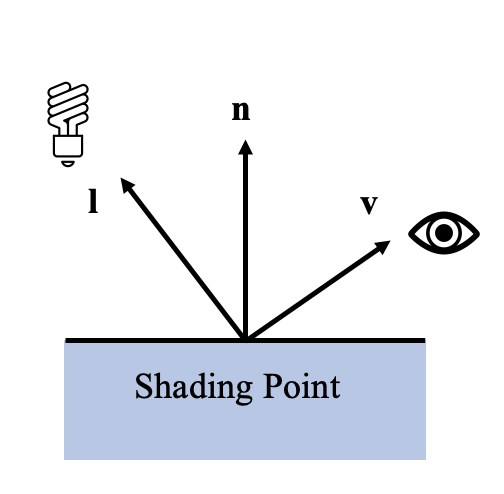
\includegraphics[scale=.6]{fanshemoxing.png}
	\caption{光线反射模型}
	\label{fig:fanshe}
\end{figure}
对于任何的着色点, 我们定义了: 
\begin{itemize}
	\item 法线$\overrightarrow{n}$, 是垂直于反射面的线; 
	\item 观察方向$\overrightarrow{v}$, 是着色点和观察点的连线; 
	\item 光照方向$\overrightarrow{l}$, 是着色点和光源的连线. 
\end{itemize}
以上的方向向量都是单位向量. 同时我们还需要定义物体表面的参数, 例如颜色, 亮度. 当我们着色时, 我们不考虑其他的物体遮挡, 因此着色中没有阴影. 

\section{漫反射}
漫反射指的是一束光线会向各个方向均匀地反射. 

\subsection{Lambert's 余弦定律}
\textbf{Lambert's 余弦定律 (Lambert's Cosine Law) }说明了漫反射光的能量和入射角度之间的关系. 光线反射的能量和光照方向和发现的夹角cos值 (向量点乘的结果) 成正比关系. 

\subsection{点光源}
我们认为光源是一个点. 在同一时刻光的能量集中在同一个球壳上. 根据能量守恒定律我们可以得知, 每一个球壳上光能量相同. 随着球壳变大, 单位面积上的光能量减小. 我们定义距离为1的光能量为$I$. 光能量和距离成平方反比关系, 距离为$r$的地方的光能量为$\frac{I}{r^2}$.

\subsection{漫反射计算公式}
漫反射能量的计算公式如下: 
\begin{equation}
	L_d = k_d\ \frac{I}{r^2}\ \text{max}(0, \textbf{n\cdot l})
\end{equation}
这里, $k_d$代表吸收率, 如果用RGB定义一个向量作为吸收率就可以代表这个反射点的颜色. $\text{max}(0, \textbf{n\cdot l})$可以把反射光线在反方向的光线过滤掉, 这些光线没有贡献. 同时, 漫发射和观察的方向无关

\section{高光 (镜面反射) }
我们认为光滑的平面可以满足基本的镜面反射的物理规律 (入射角等于反射角) . 当我们的观察方向和反射角方向一直的时候就可以看到高光. 我们一般使用半程向量和法线的接近程度来“映射”观察方向和反射角的接近程度. 半程向量指的是光源方向和观察方向角平分线上的方向向量. 
\begin{equation}
	\textbf{h} = \text{bisector}(\textbf{v}, \textbf{l}) = \frac{\textbf{v} + \textbf{l}}{||\textbf{v} + \textbf{l}||}
\end{equation}
高光的计算公式如下: 
\begin{equation}
	L_s = k_s\ \frac{I}{r^2}\ \text{max}(0, \textbf{n\cdot h})^p
\end{equation}
一边来说高光的颜色$k_s$为白色. 我们会给cos项乘一个指数$p$. 原因是余弦函数的容忍度很高, 但是我们希望当角度偏离一点点的时候就看不到高光. 因此会使用一个指数, 一般来说$p\in [100,200]$. 
\begin{figure}[H]
	\centering
	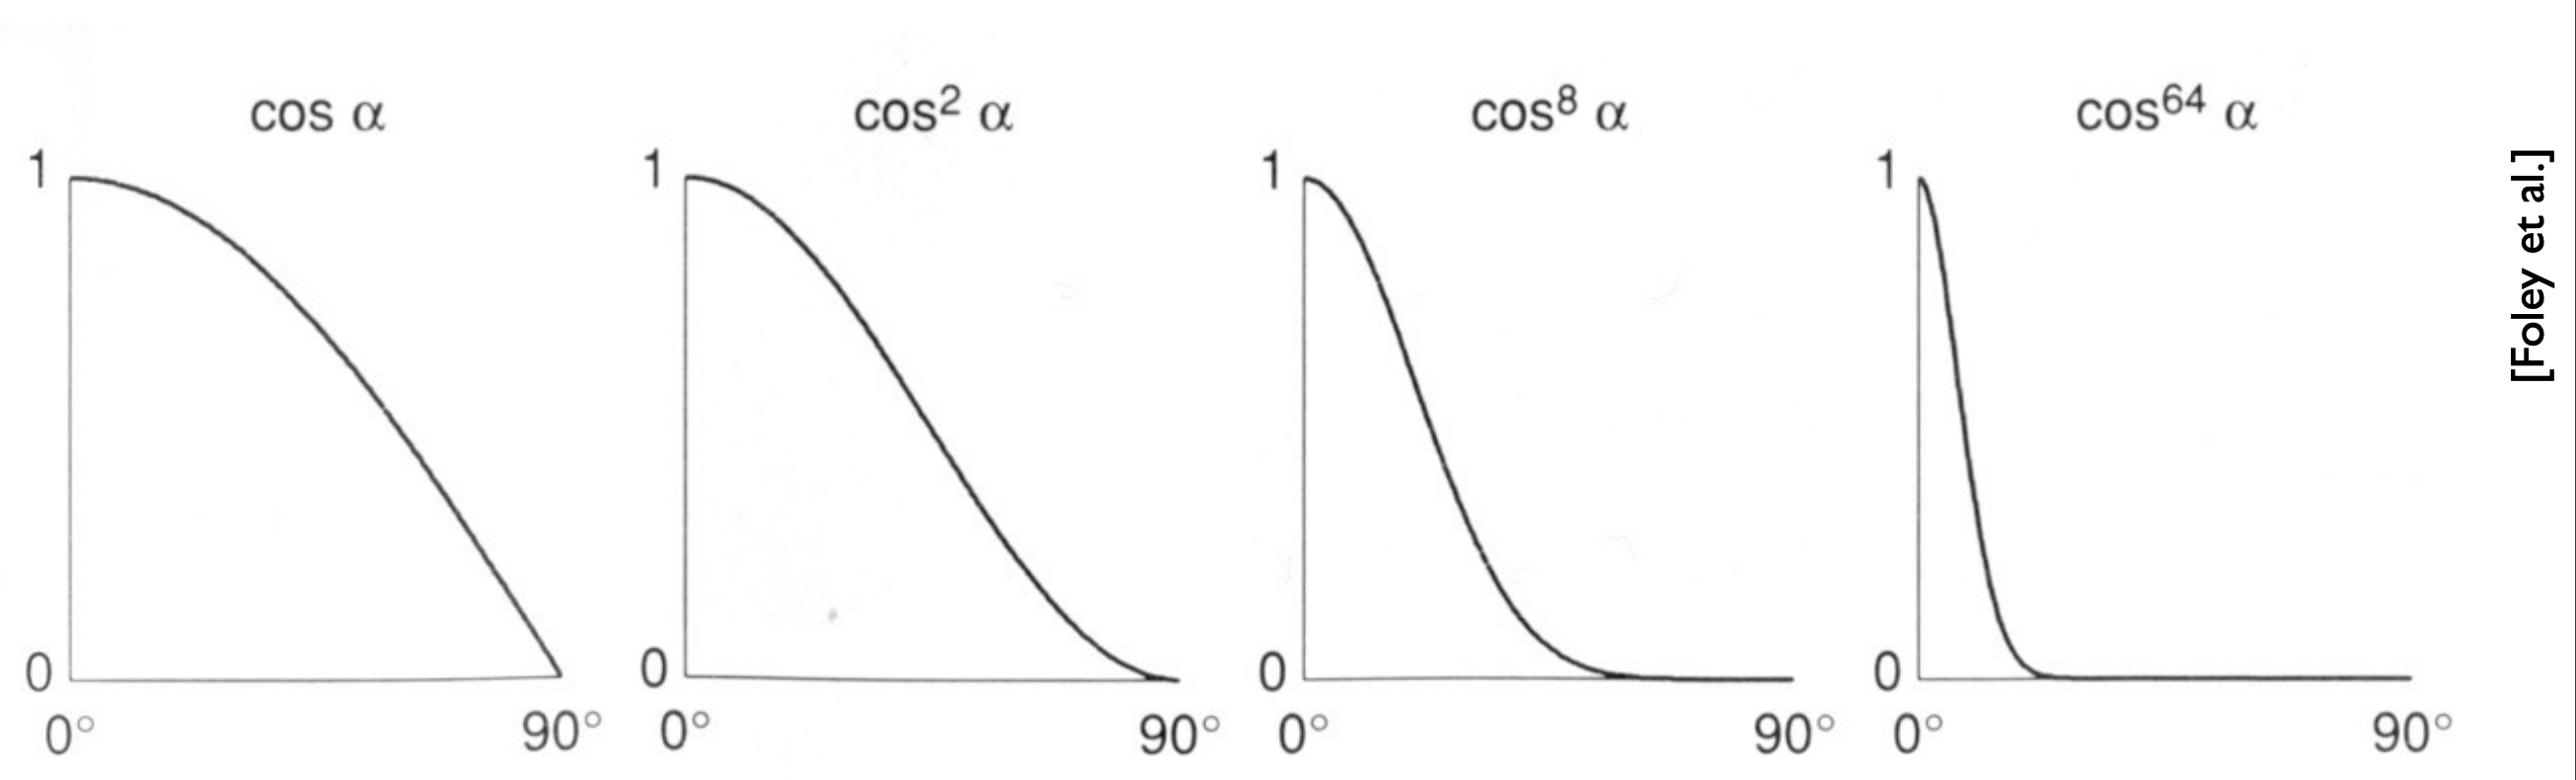
\includegraphics[scale=.2]{cos.png}
	\caption{指数的选择}
	\label{fig:cos}
\end{figure}

\section{环境光照}
我们粗略的认为环境中所有点的光照相同, 是一个常数. 环境光与光源方向, 法线方向和观察方向无关. 计算公式如下: 
\begin{equation}
	L_a = k_a\ I_a
\end{equation}

\section{Blinn-Phong反射模型}
综上所述, Blinn-Phong反射模型可以表示为: 
\begin{equation}
	L = L_a + L_d + L_s = k_a\ I_a +  k_d\ \frac{I}{r^2}\ \text{max}(0, \textbf{n\cdot l}) + k_s\ \frac{I}{r^2}\ \text{max}(0, \textbf{n\cdot h})^p
\end{equation}
\begin{figure}[H]
	\centering
	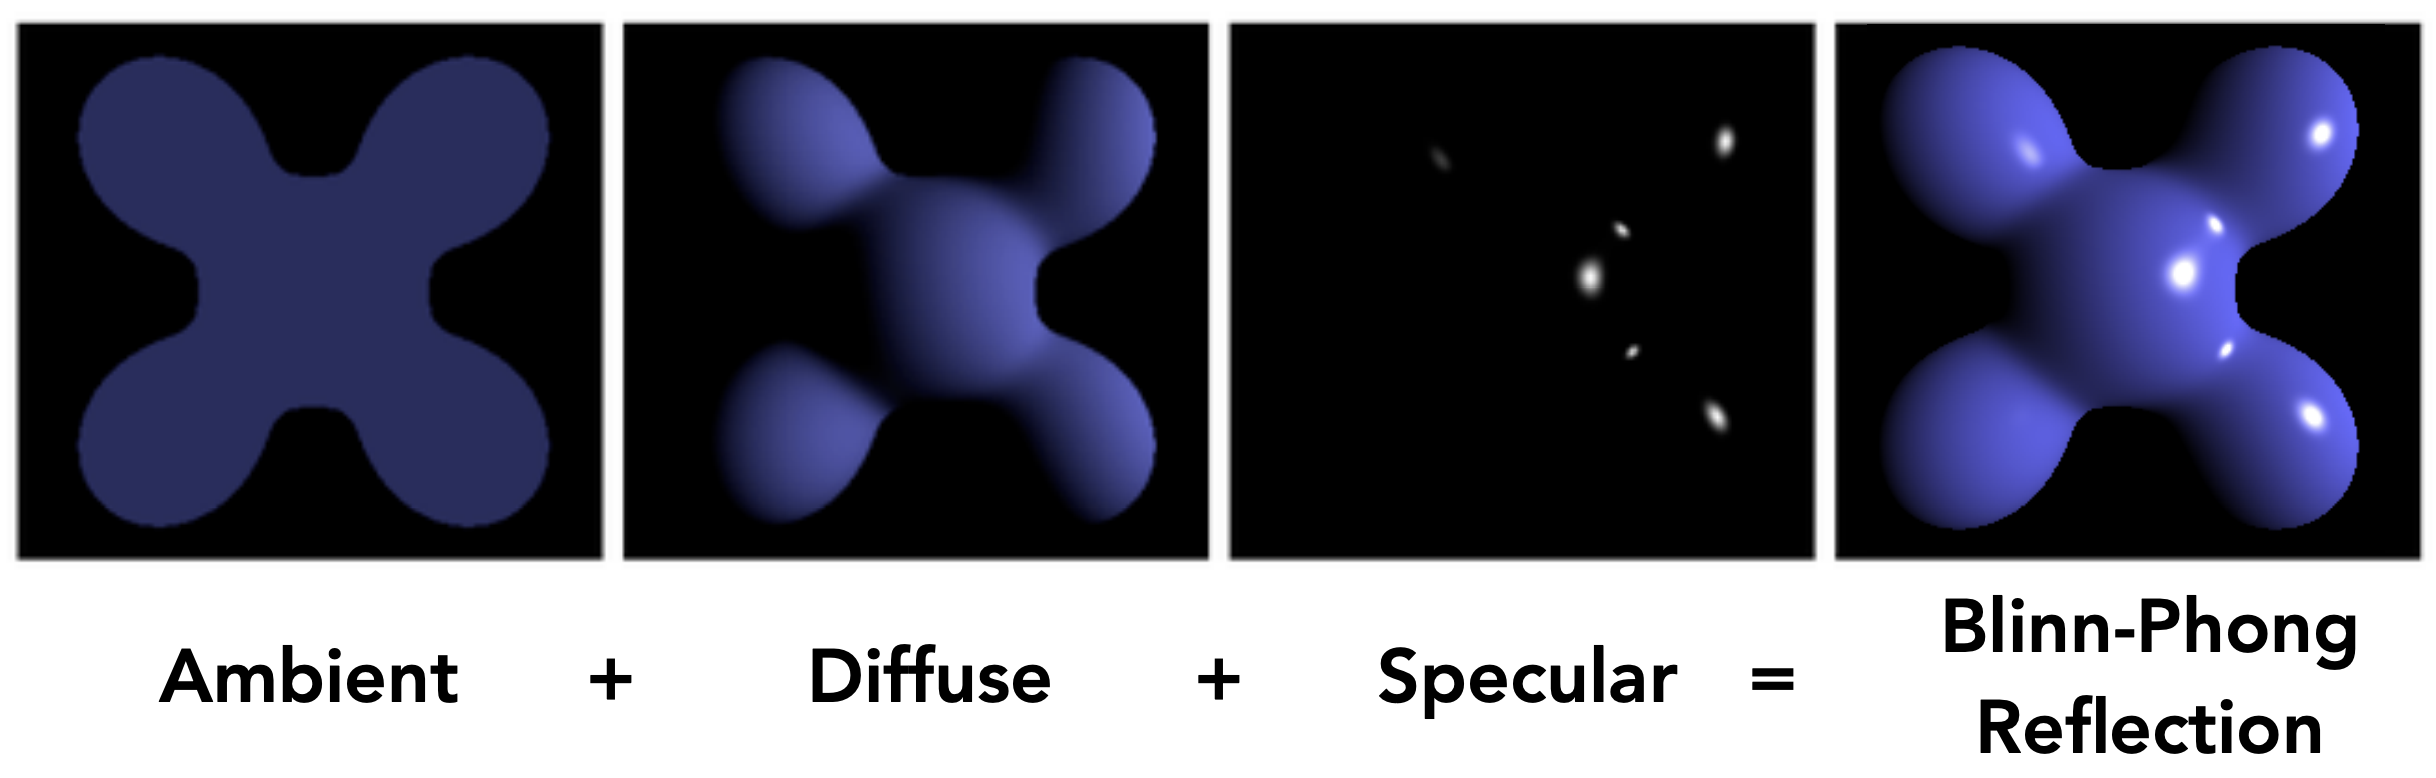
\includegraphics[scale=.3]{phonemodel.png}
	\caption{Blinn-Phong反射模型}
	\label{fig:phonemodel}
\end{figure}

\chapter{着色频率和管线}

\section{着色频率}
根据不同的着色方式, 有不同的着色频率, 主要的着色频率分为三种——面着色, 顶点着色和像素着色. 主要的不同之处在于法线的选择方式不同. 

\begin{itemize}
	\item \textbf{面着色 (Flat Shading) }指的是计算每一个三角形平面的法线后对一个平面整体进行着色; 
	\item \textbf{顶点着色 (Gouraud Shading) }指的是计算每一个三角形三个顶点的法线后进行着色, 最后在三角形内部插值得到颜色. 顶点法线的计算是通过顶点相邻面的法线的 (加权) 平均值求出; 
	\item \textbf{像素着色 (Phong Shading) }指的是计算出每一个像素的法线进行着色. 三角形内部点法线的计算需要依靠重心坐标计算. 
\end{itemize}
当几何体相对复杂, 构造精细的时候, 三种着色效果产生的结果不相上下. 

\section{ (实时渲染) 管线}
\textbf{管线 (Pipeline) }是从模型到图片生成的过程. 管线分为以下过程: 
\begin{figure}[H]
	\centering
	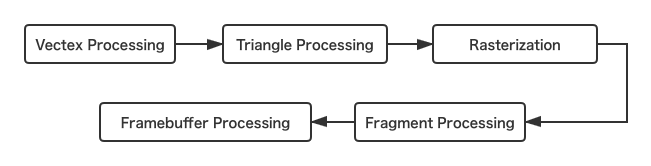
\includegraphics[scale=.6]{pipeline.png}
	\caption{管线}
	\label{fig:pipeline}
\end{figure}

首先将顶点的三位向量作为输入, 进行几何变换后划分三角形区域. 通过光栅化获得一个个小的碎片 (或者是一个个小像素) 后进行着色, 得到我们的输出. 

我们可以定义顶点或者像素的着色方式来提供不同的着色要求, 这被称为\textbf{Shader}. 硬件中会提供这样的编程方式定制不同的着色方式, 以OpenGL为例, 我们可以定义以下的着色函数: 
\begin{lstlisting}
uniform sampler2D myTexture;
uniform vec3 lightDir;
varying vec2 uv;
varying vec3 norm;

void diffuseShader(){
	vec3 kd;
	kd = texture2d(myTexture, uv);
	kd *= clamp(dot(-lightDir, norm), 0.0, 1.0);
	gl_FragColor = (kd, 1.0);
}
\end{lstlisting}
这里我们定义了一个简单的漫反射着色器. 同时, 着色器会自动应用到每一个顶点或者是像素上, 不需要我们使用显式的for循环进行遍历. 

\begin{information}
	我们可以进入Shadertoy网站 (\url{https://www.shadertoy.com/view/ld3Gz2}) 练习Shader编程, 编程的结果会直接显示在网页中. 
\end{information}

\chapter{纹理映射}

对于任何一个三角形, 我们在内部填充一个图形作为纹理. \textbf{纹理 (Texture) }也就是我们在不同的位置所定义的漫反射系数. 

\section{三维物体表面展开}

任何一个三维物体的表面都是二维的图形, 我们可以将一个三维物体表面映射到一个二维的图像上. 图形的映射非常的复杂, 这里不做过多解释. 我们将纹理建立一个$u-v$坐标系. 同时$u,v\in[0,1]$. 

当然, 我们在为墙面, 地面加入纹理的时候可以使用边缘连接连续的纹理, 称为\textbf{tiled}. 这样子就可以复用纹理拼接大表面. 我们可以知道每一个三角形的顶点坐标和对应的纹理坐标, 那么我们怎么求出来三角形内部顶点坐标对应的纹理坐标. 这就是一个插值问题, 我们需要使用重心坐标的方式计算. 

\section{重心坐标}
我们在之前的节中留下了以下疑问, 已知三角形三个顶点的颜色, 法线或者纹理坐标, 如何求出三角形内部某一点对应的插值量?这个时候我们就需要使用\textbf{重心坐标 (Barycentric Coordinate) }来计算. 

对于$\triangle ABC$内任意一点$(x,y)$可以满足: 
\begin{equation}
	\begin{split}
		&(x,y) = \alpha A + \beta B + \gamma C, \\
		&\alpha + \beta + \gamma = 1,\\
		& \alpha, \beta, \gamma >= 0
	\end{split}
\end{equation}
三角形平面上的任意一点都可以用三角形三个顶点坐标的线性组合表示. 三角形内部的点必须满足系数加和为1并且系数均为非负数. 那么重心坐标就是$(\alpha,\beta,\gamma)$, 已知任意两个重心坐标可以直接推断出第三个坐标. 
重心坐标可以通过面积求出, 我们令三角形内一点和三个顶点相连, 每一个顶点所对的小三角形的面积为$A_A,A_B,A_C$, 那么重心坐标可以用以下方式计算: 
\begin{figure}[H]
	\centering
	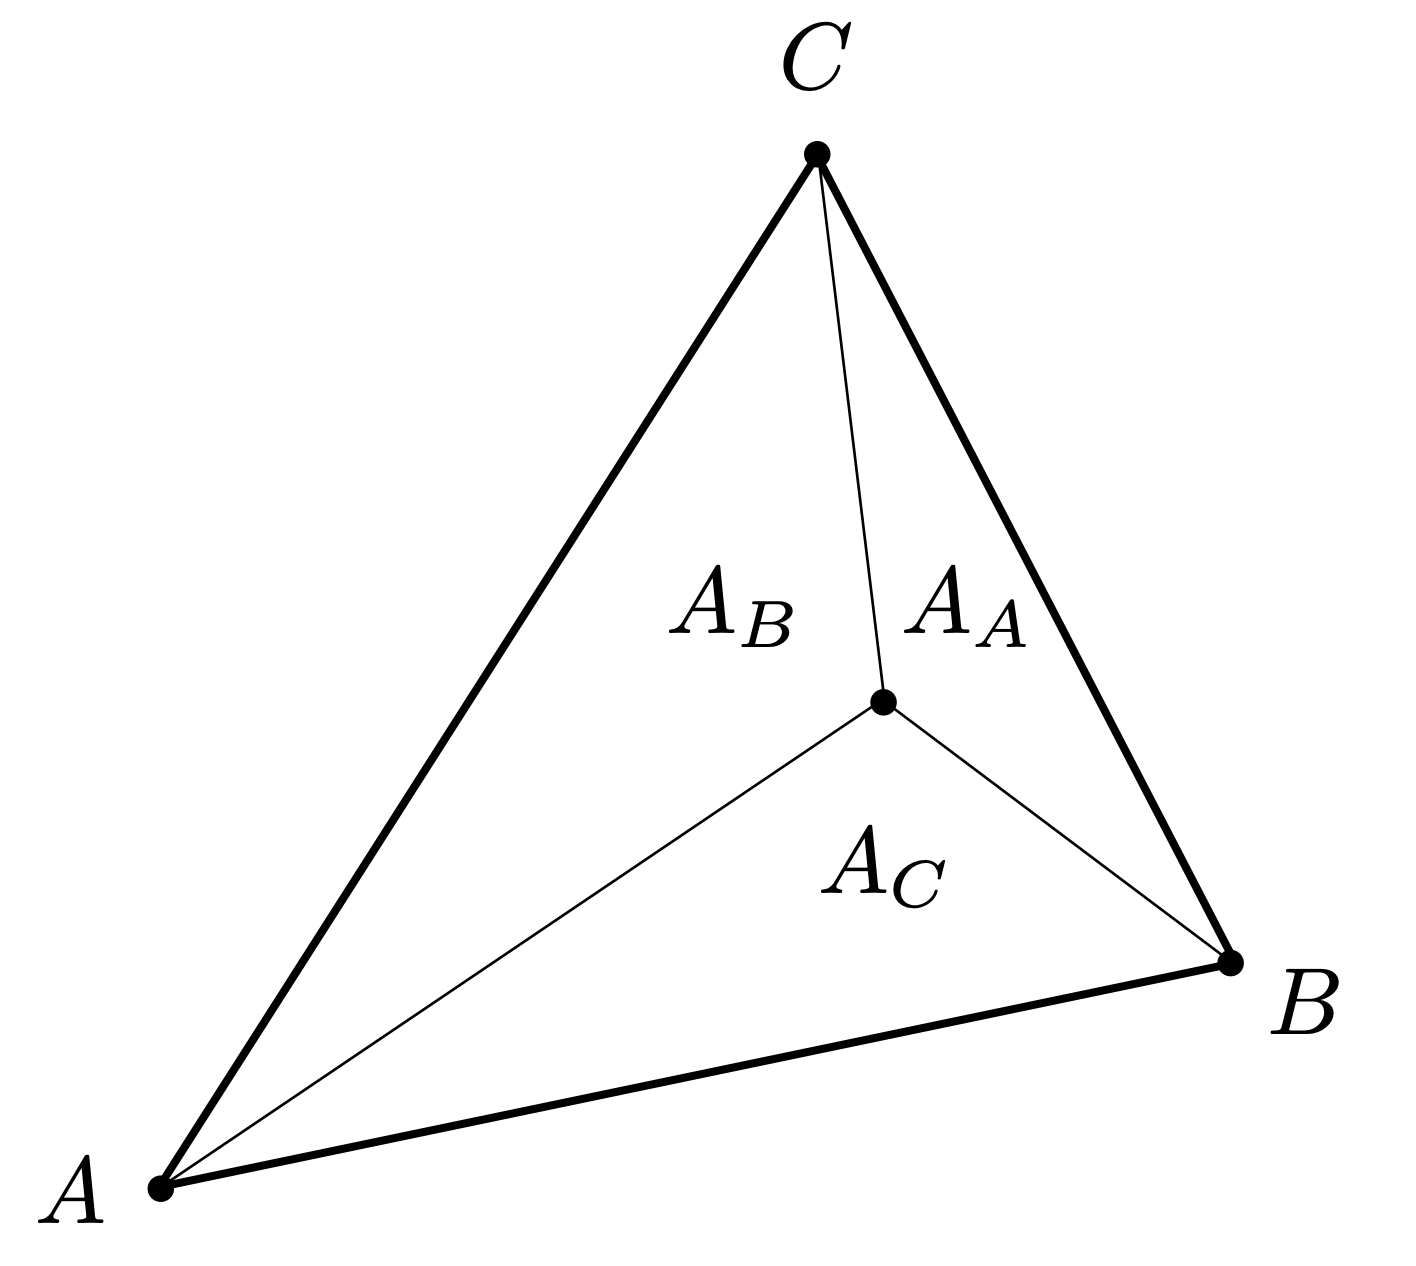
\includegraphics[scale=.15]{zhongxinzuobiao.png}
	\caption{重心坐标的计算}
	\label{fig:zongxinzuobiao}
\end{figure}
\begin{equation}
	\begin{split}
		\alpha = \frac{A_A}{A_A+A_B+A_C},\\
		\beta = \frac{A_B}{A_A+A_B+A_C},\\
		\gamma = \frac{A_C}{A_A+A_B+A_C}\\
	\end{split}
\end{equation}
当重心坐标为$(\frac{1}{3},\frac{1}{3},\frac{1}{3})$的时候, 这个点是三角形的重心. 已知三个顶点的坐标也可以直接推算出重心坐标: 
\begin{equation}
	\begin{split}
		&\alpha = \frac{-(x-x_B)(y_C-y_B) + (y-y_B)(x_C-x_B)}{-(x_A-x_B)(y_C-y_B) + (y_A-y_B)(x_C-x_B)},\\
		&\beta =  \frac{-(x-x_C)(y_A-y_C) + (y-y_C)(x_A-x_C)}{-(x_B-x_C)(y_A-y_C) + (y_B-y_C)(x_A-x_C)},\\
		&\gamma = 1-\alpha-\beta\\
	\end{split}
\end{equation}

如果三角形三个顶点对应了三个向量 (颜色, 法线或者纹理坐标) , 那么内部点对应的向量值是使用重心坐标进行的线性组合. 假设三个顶点对应的向量是$V_A,V_B,V_C$, 那么三角形中任意一点的插值后向量是$V=\alpha V_A +\beta V_B+\gamma V_C$. 同时, 重心坐标在投影后不能保证结果不变, 因此我们在空间中需要使用三维坐标计算的重心坐标来进行插值. 

\section{纹理映射的问题}
纹理映射主要分为两步, 第一步是把像素点坐标映射到纹理坐标$(x,y)\rightarrow (u,v)$. 第二部根据纹理坐标得到对应的漫反射系数$(u,v)\rightarrow k_d$, 纹理上的像素叫做纹理元素或者纹素 (Texel) . 但是如果纹理过大或者过小都会出现一些问题. 

\textbf{如果纹理太小的话......}

如果纹理本身太小, 但是物体像素点比较多, 那么就会产生非常多类似于马赛克的像素. 这是由于很多像素点会求出浮点数纹理坐标, 在取整后会导致马赛克的产生. 我们用两种方式解决, 一种是双线性插值法, 另一种是二次样条插值法. 
\begin{figure}[H]
	\centering
	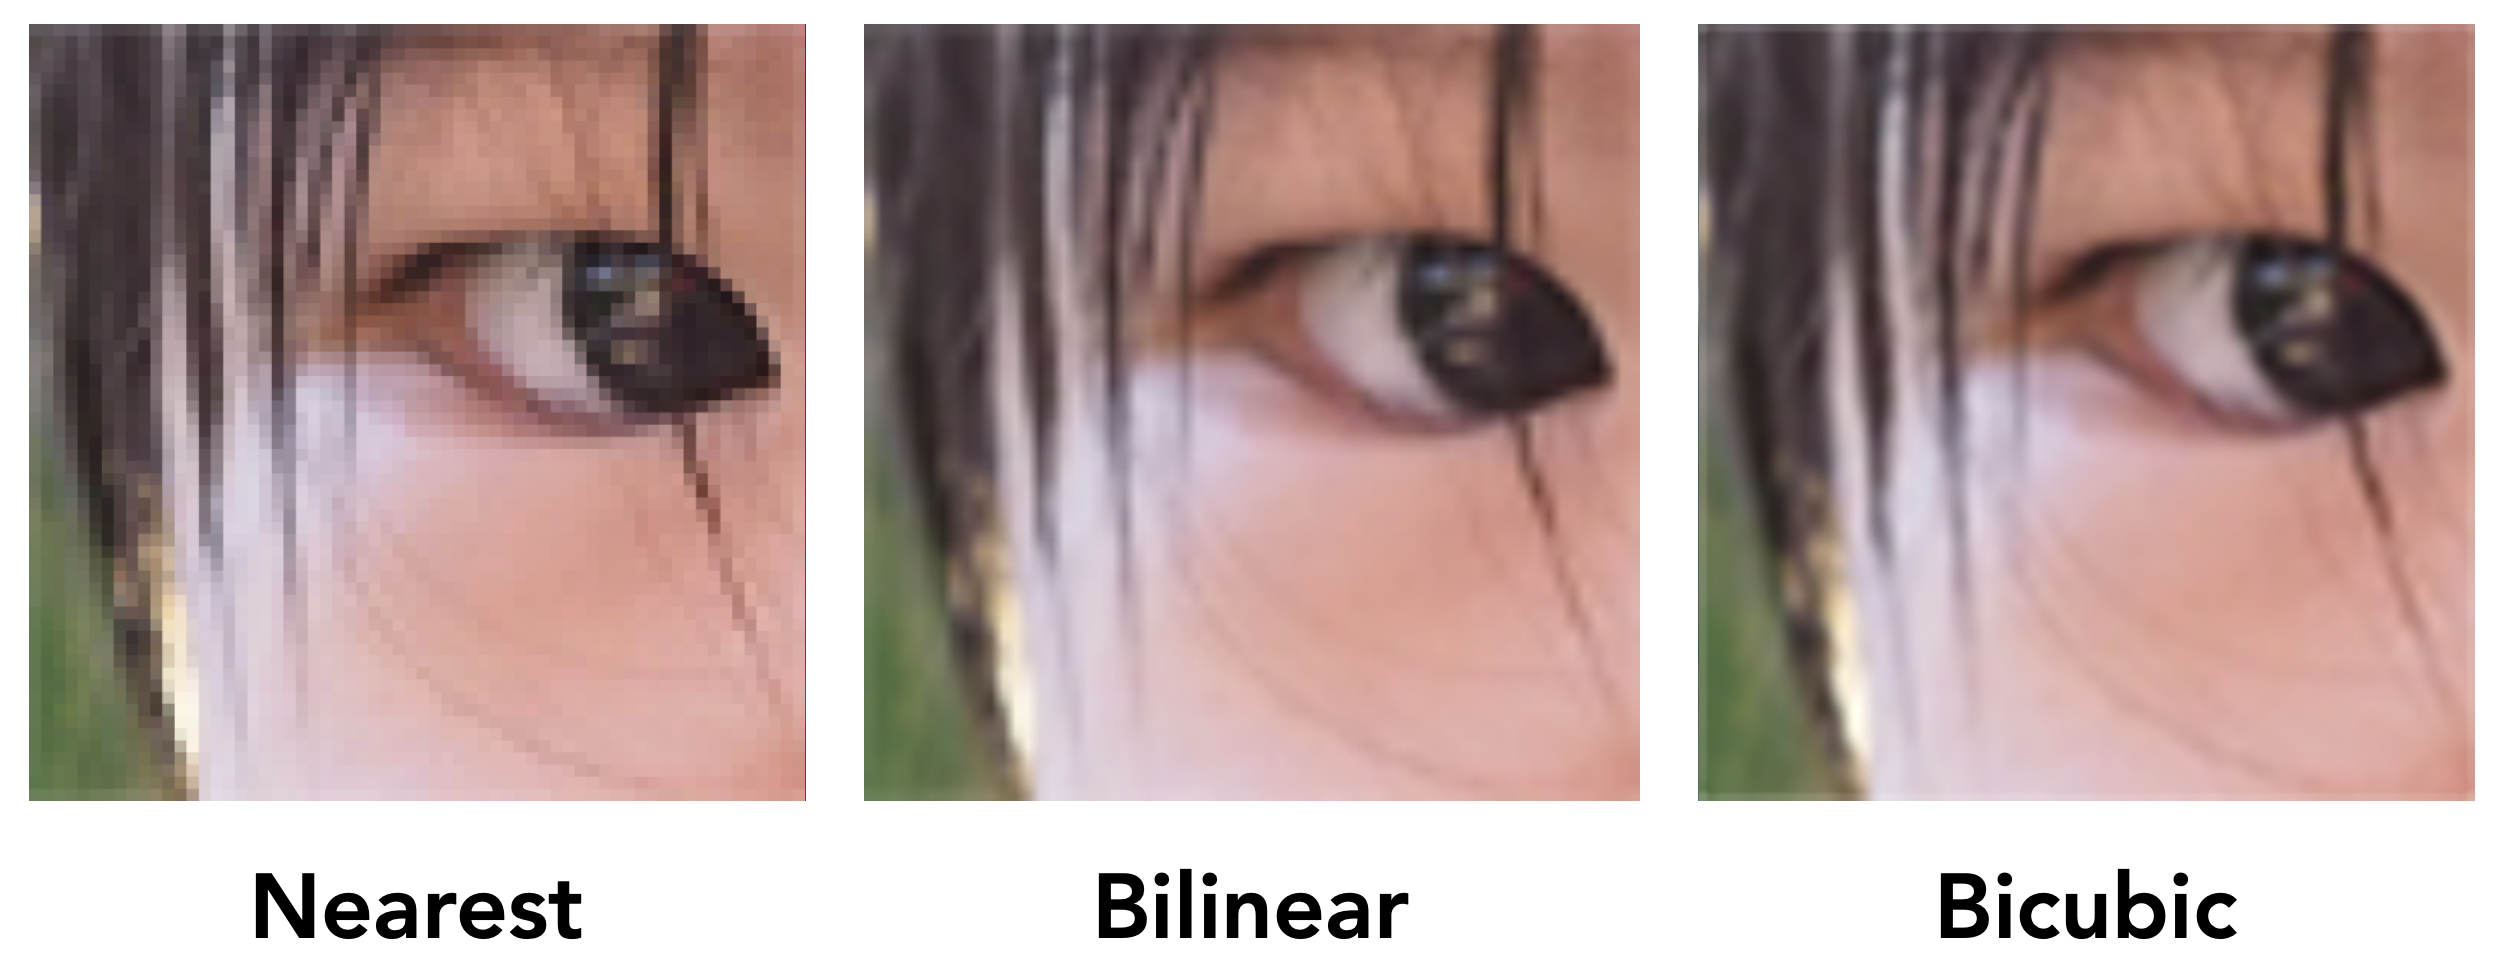
\includegraphics[scale=.25]{chazhi.png}
	\caption{纹理过小的解决方案}
	\label{fig:chazhi}
\end{figure}

\textbf{双线性插值 (Bilinear Interpolation) }指的是对于任意一个纹理坐标, 我们使用其临近的四个纹素值进行两次线性插值得到这个坐标对应的漫反射率. 

\begin{figure}[H]
	\centering
	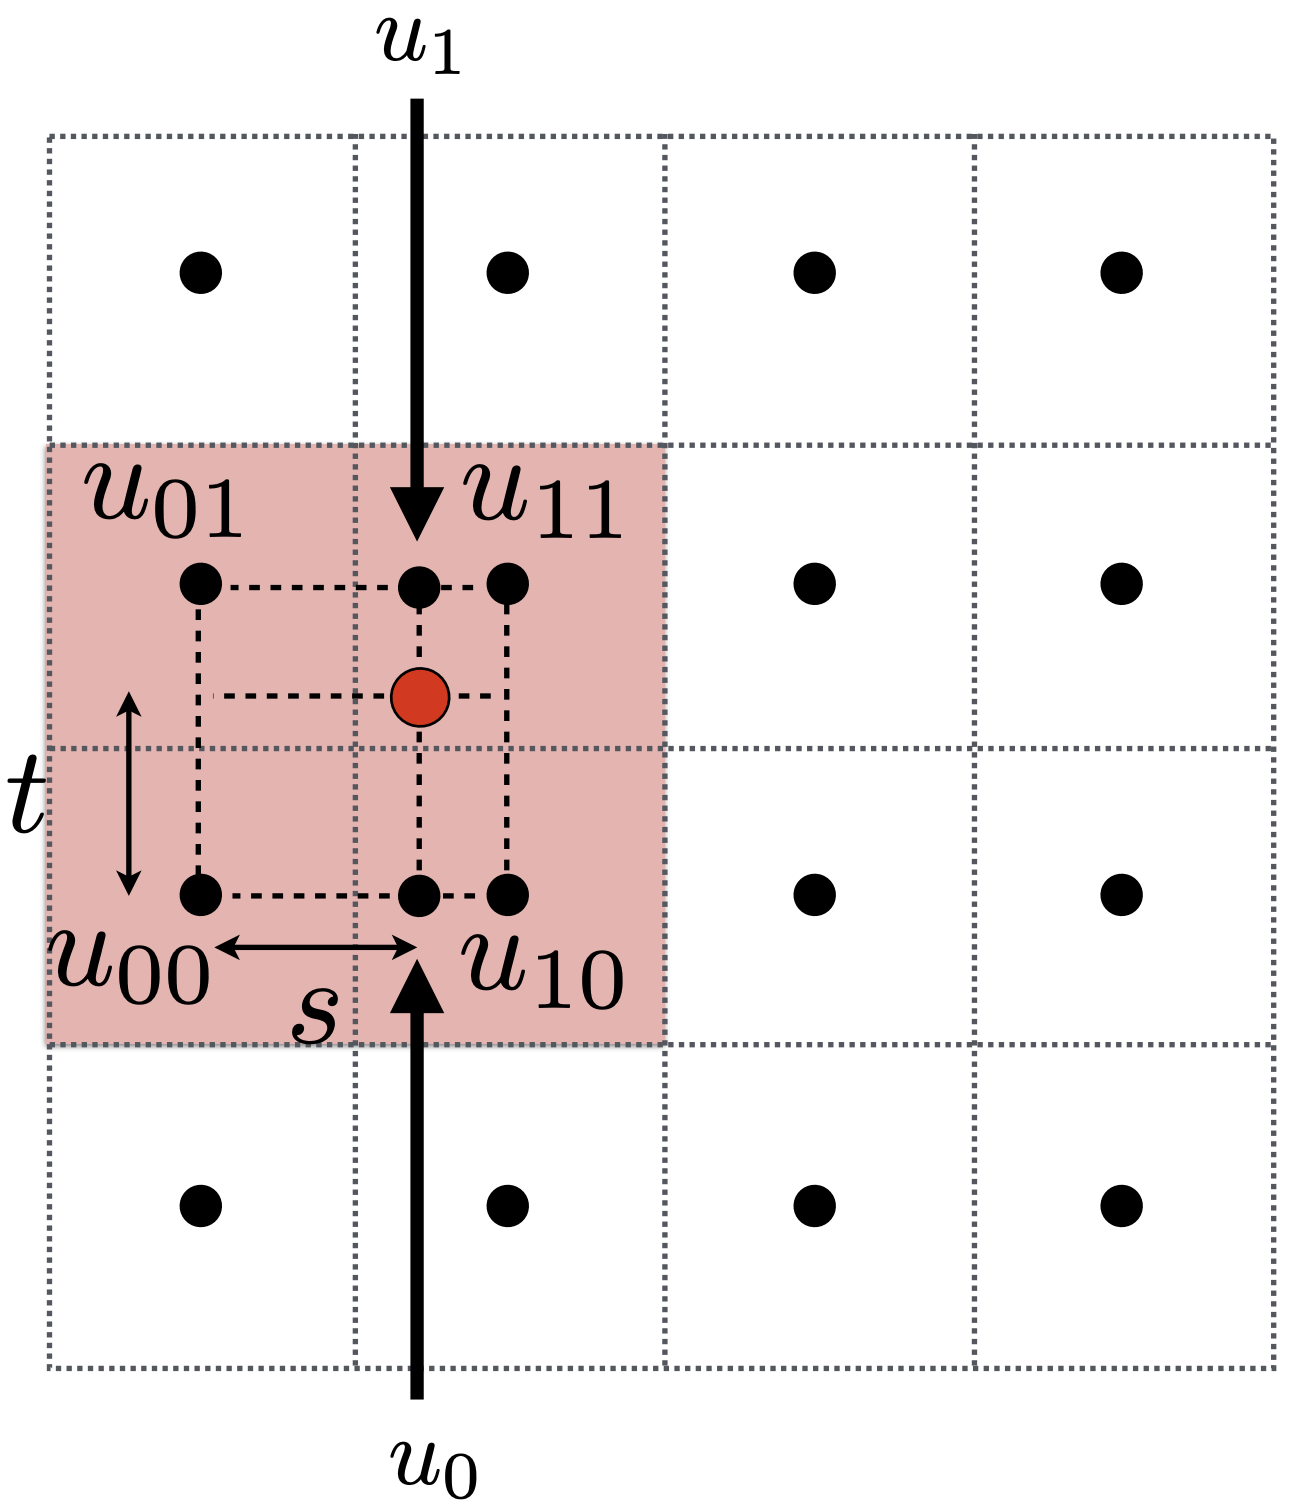
\includegraphics[scale=.15]{shuangxianxing.png}
	\caption{双线性插值示意图}
	\label{fig:shuangxianxing}
\end{figure}
在一维上的线性插值可以表示为: $\text{lerp}(x,v_0,v_1)=v_0+x(v_1-v_0)$. 首先我们在水平方向上做两次线性插值: 
\begin{equation}
	\begin{split}
		u_0 = \text{lerp}(s,u_{00},u_{10})\\
		u_1 = \text{lerp}(s,u_{01},u_{11})\\
	\end{split}
\end{equation}
然后我们在纵向上做一次线性插值: 
\begin{equation}
		f(x,y) = \text{lerp}(s,u_{0},u_{1})\\
\end{equation}
插值的结果相比于之前变化更加顺畅. 

\textbf{双立方插值 (Bicubic Interpolation) }使用相邻16个点进行计算, 效果更好但是计算量相对来说更大. 

\textbf{如果纹理太大的话......}

当纹理过大的时候, 近处的物体会产生锯齿, 远处的物体会产生摩尔纹, 也就是说结果会产生走样. 主要原因是因为当物体离得越远, 每一个像素所代表的纹素的数量会变多. 这个时候再使用像素和纹素一一对应的方式是不可靠的. 
\begin{figure}[H]
	\centering
	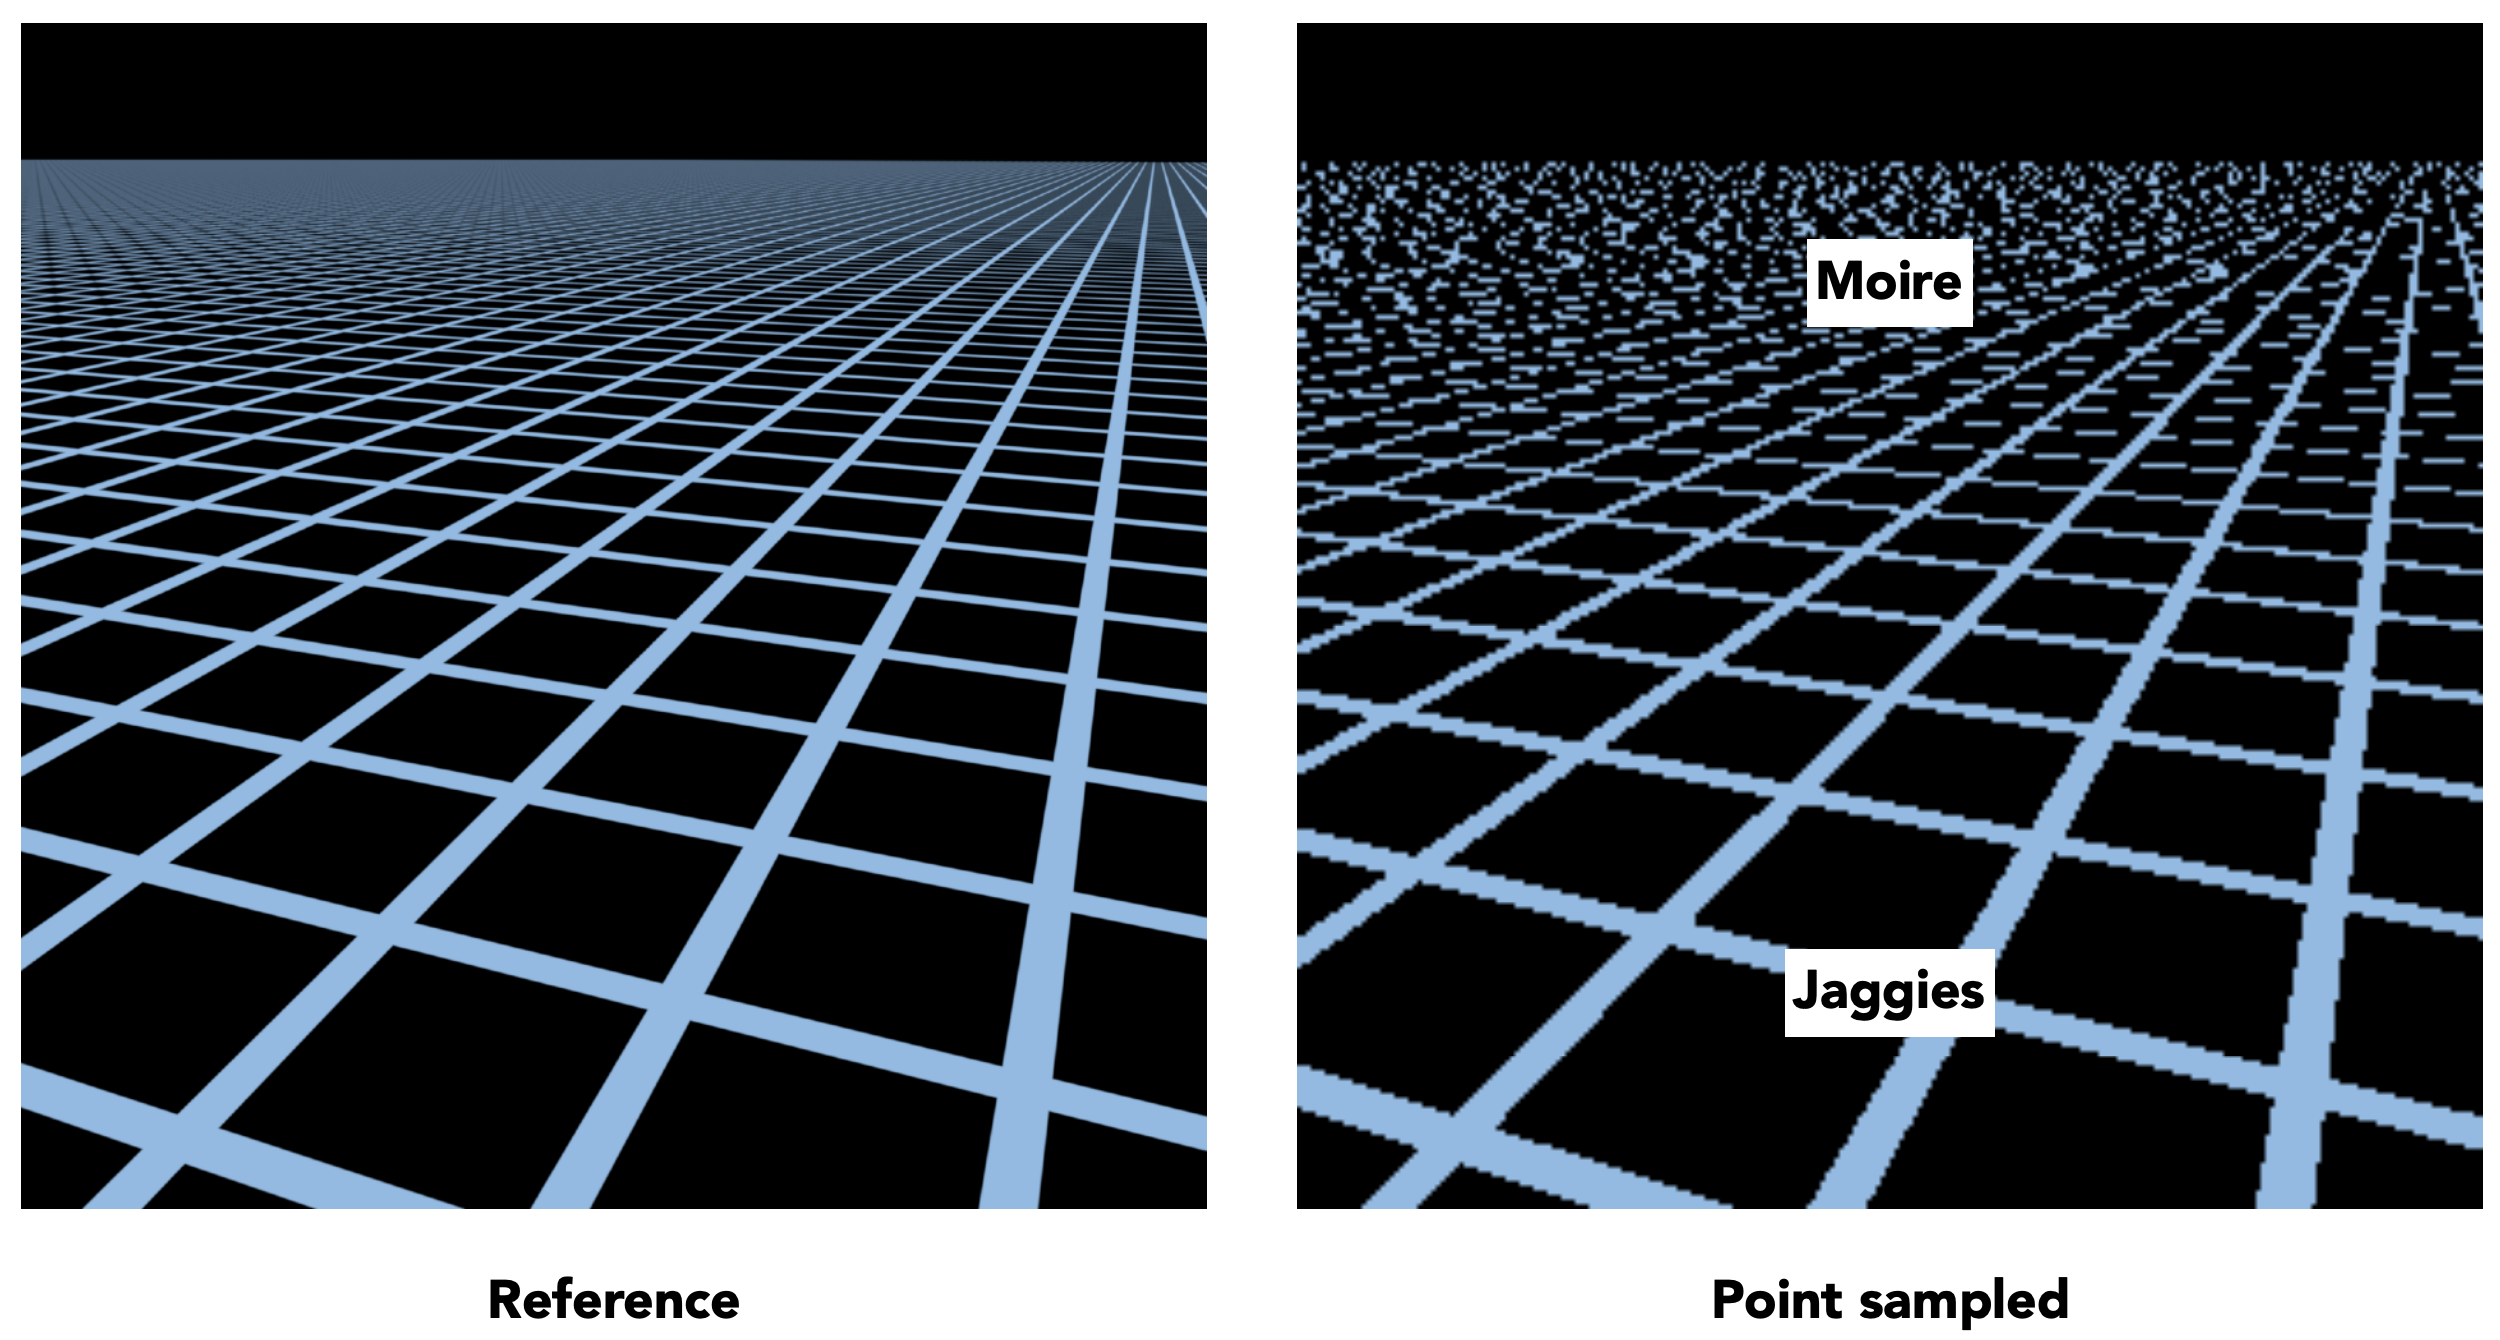
\includegraphics[scale=.15]{dawenli.png}
	\caption{纹理过大结果示意图}
	\label{fig:dawenli}
\end{figure}
我们的解决方法是避免采样. 通过像素点直接得到对应纹素区域的平均值. 这里我们引入\textbf{Mipmap}来解决这样一个范围查询的问题. Mipmap是一个快速, 近似并且只用于正方形区域的范围查询方法. 主要思想如下: 我们从一张纹理生成一系列的纹理. 每一个纹理的大小都是之前纹理大小的一半, 最后得到的最小的纹理是一个$1\times 1$的纹理, 这就是一个图像金字塔. 最终存储这些纹理额外的开销是原本纹理的三分之一. 

我们需要计算每一个像素对应纹理的方形大小, 并使用对应层的纹理. 
\begin{figure}[H]
	\centering
	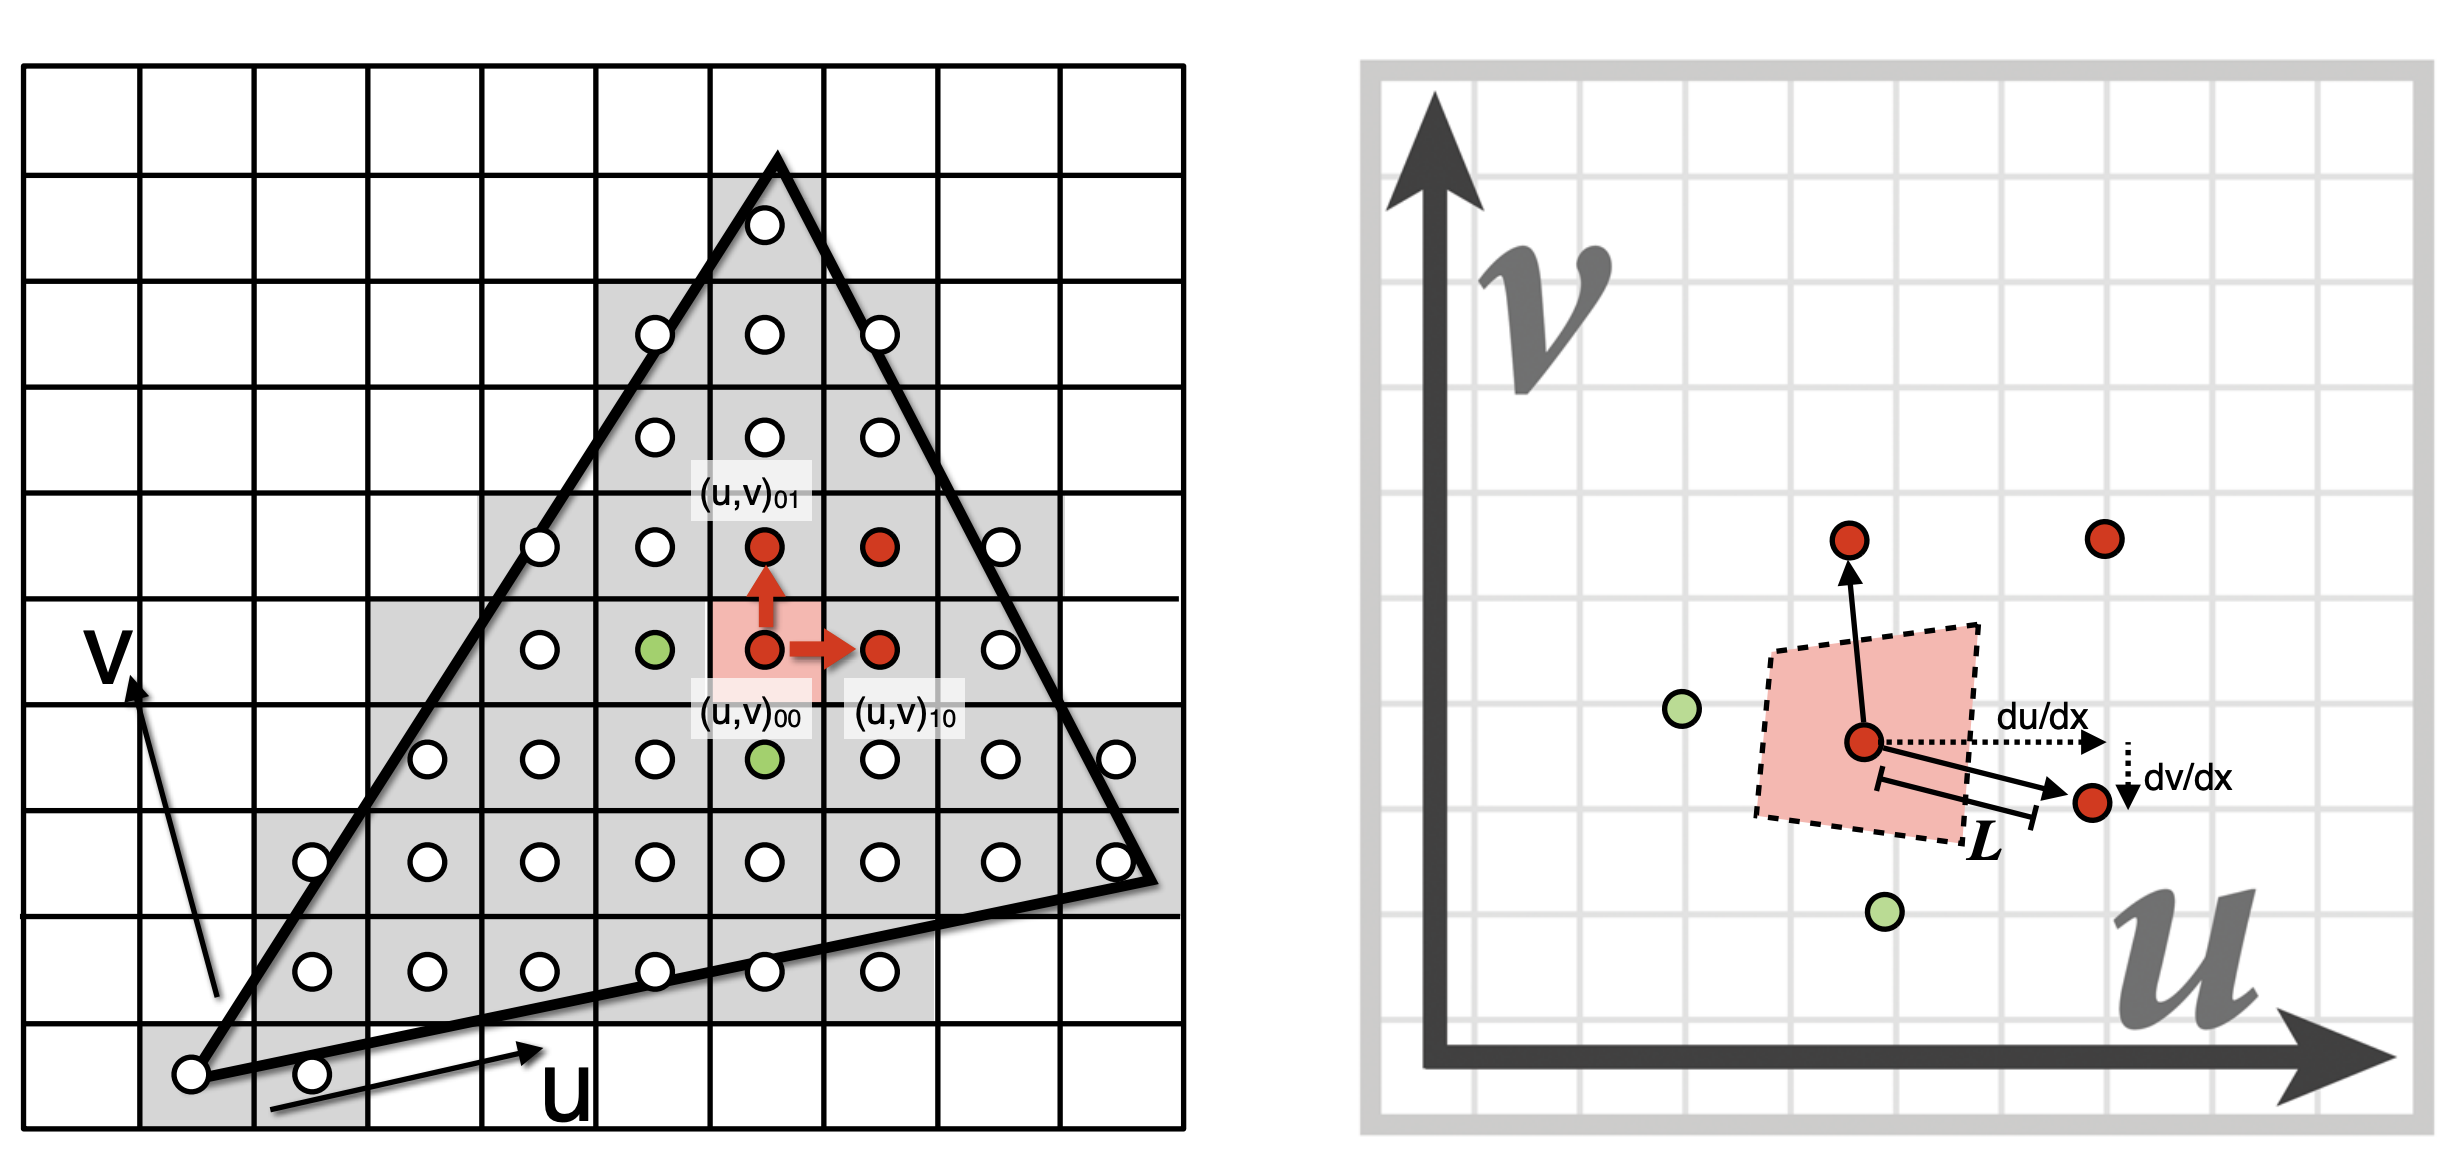
\includegraphics[scale=.3]{mipmap.png}
	\caption{Mipmap对应层数计算}
	\label{fig:mipmap}
\end{figure}
对于一个点$u(0,0)$何其相邻的两个点之间在纹理上的距离, 可以用微分形式表示, 那么这个像素所对应纹理方形的大小是: 
\begin{equation}
	L= \text{max}(\sqrt{(\frac{du}{dx})^2+(\frac{dv}{dx}^2)},\sqrt{(\frac{du}{dy}^2)+(\frac{dv}{dy}^2)})
\end{equation}
那么对应的层数为: $D=\log_2L$. 
为了保证我们能够取到的层数是一个连续的层数, 我们使用三线性插值法得到对应的结果. 首先, 对于任意一个非整数层数, 我们在其上下两层使用双线性插值进行取值. 接下来我们在两个层之间使用线性插值就可以得到最后的结果. 

Mipmap也存在局限性. 由于所有的纹理都必须对应到一个正方形的区域, 但是并不是所有的纹理都可以被一个正方形完美的包住 (例如细长的长方形, 或者是在对角线上的长方形) . 最终远处的纹理会变得非常的模糊, 丢失了许多细节. 
\begin{figure}[H]
	\centering
	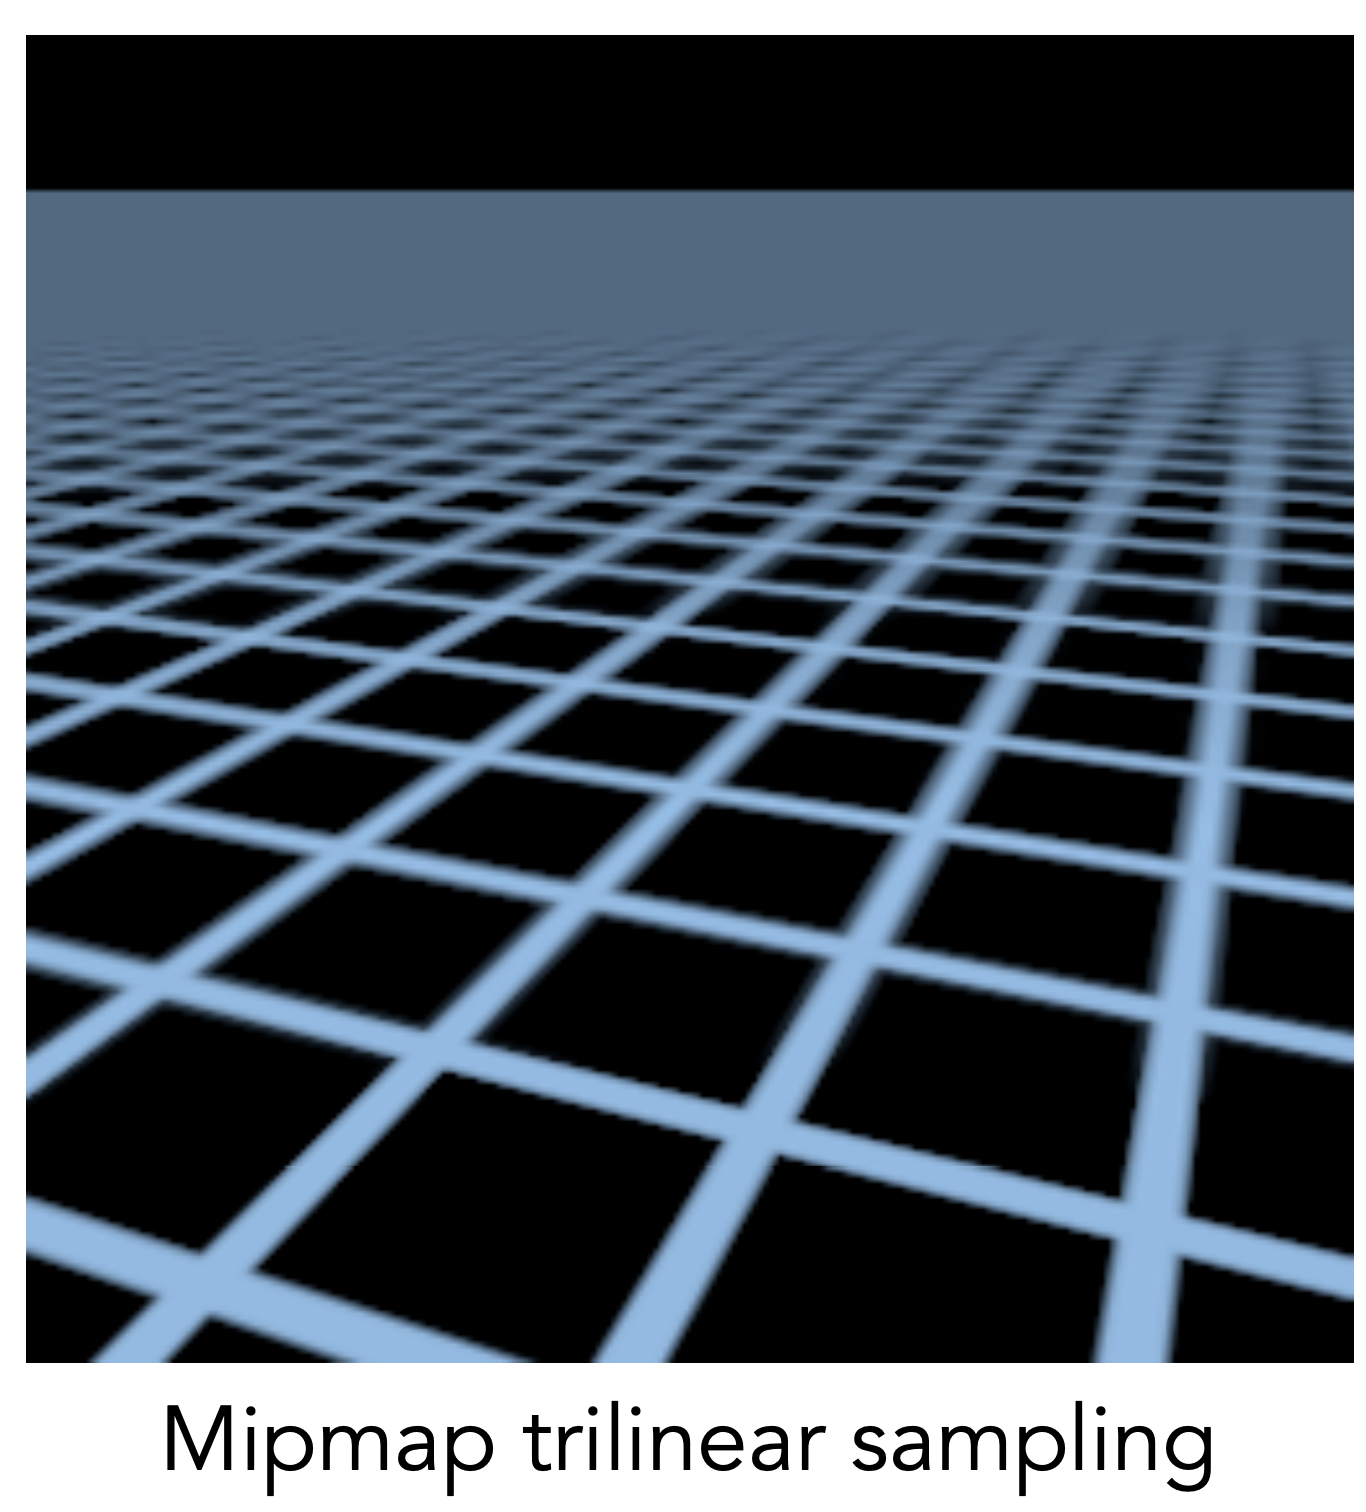
\includegraphics[scale=.2]{mipmapjuxian.png}
	\caption{Mipmap的局限性}
	\label{fig:mipmapjuxian}
\end{figure}
为了解决这个问题, 我们使用\textbf{各向异性过滤 (Anisotropic Filtering) }解决. 各向异性过滤指的是加入只在水平方向或者竖直方向上缩小的纹理, 这样可以应对不同长方形纹理块区域. 但是对于对角线上的纹理块依然不好解决. 并且存储多余的纹理需要多使用原来纹理三倍的开销. 
\begin{figure}[H]
	\centering
	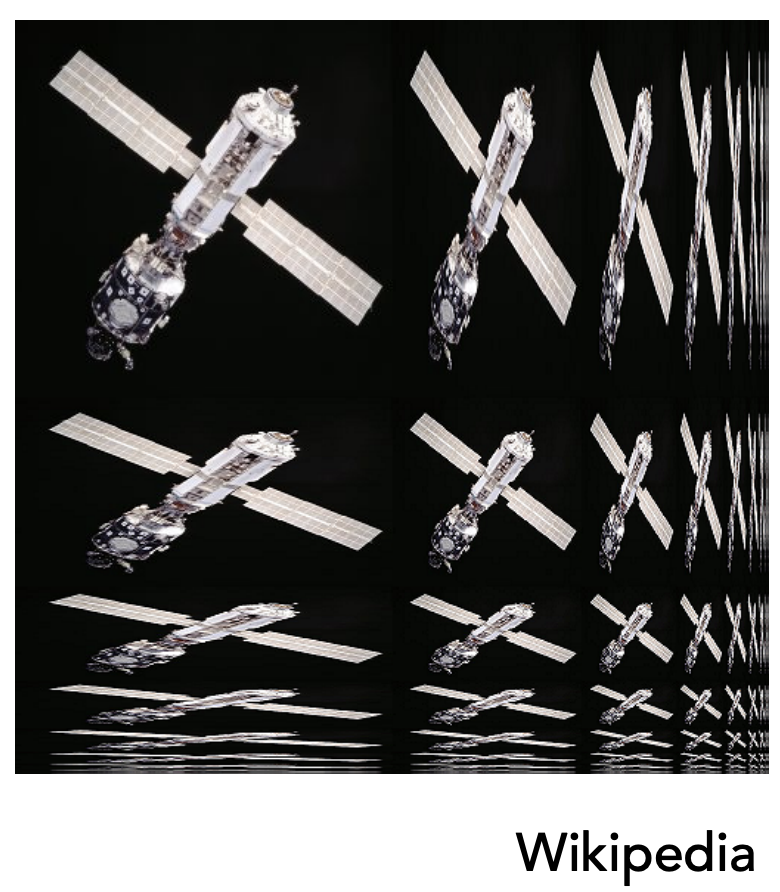
\includegraphics[scale=.3]{gexiangyixing.png}
	\caption{各向异性过滤的纹理图}
	\label{fig:gexiangyixing}
\end{figure}
除此之外我们还可以使用EWA过滤得到更好的结果. 可以把纹理拆分成不同的圆形块进行多次查询获得最终的结果. 但是开销也会比较大. 

\section{纹理的应用}
纹理除了我们所认为是一个“贴图”之外, 纹理还有各种各样的应用. 纹理是一块内存加上范围查询 (滤波) 的结果. 除了上面简单的纹理应用之外, 我们还可以使用纹理做以下事情. 

\subsection{环境贴图}
\textbf{环境贴图 (Environment Map) }指的是环境中四面八方的情况. 可以使用纹理来描述环境光的样子. 我们假设环境光来自于无穷远处, 没有深度意义. 环境光纹理可以看作一个光滑镜面的球表面在环境中所记录的信息. 我们需要将球表面展开成一个平面, 可以使用两种展开方式: 
\begin{figure}[H]
	\centering
	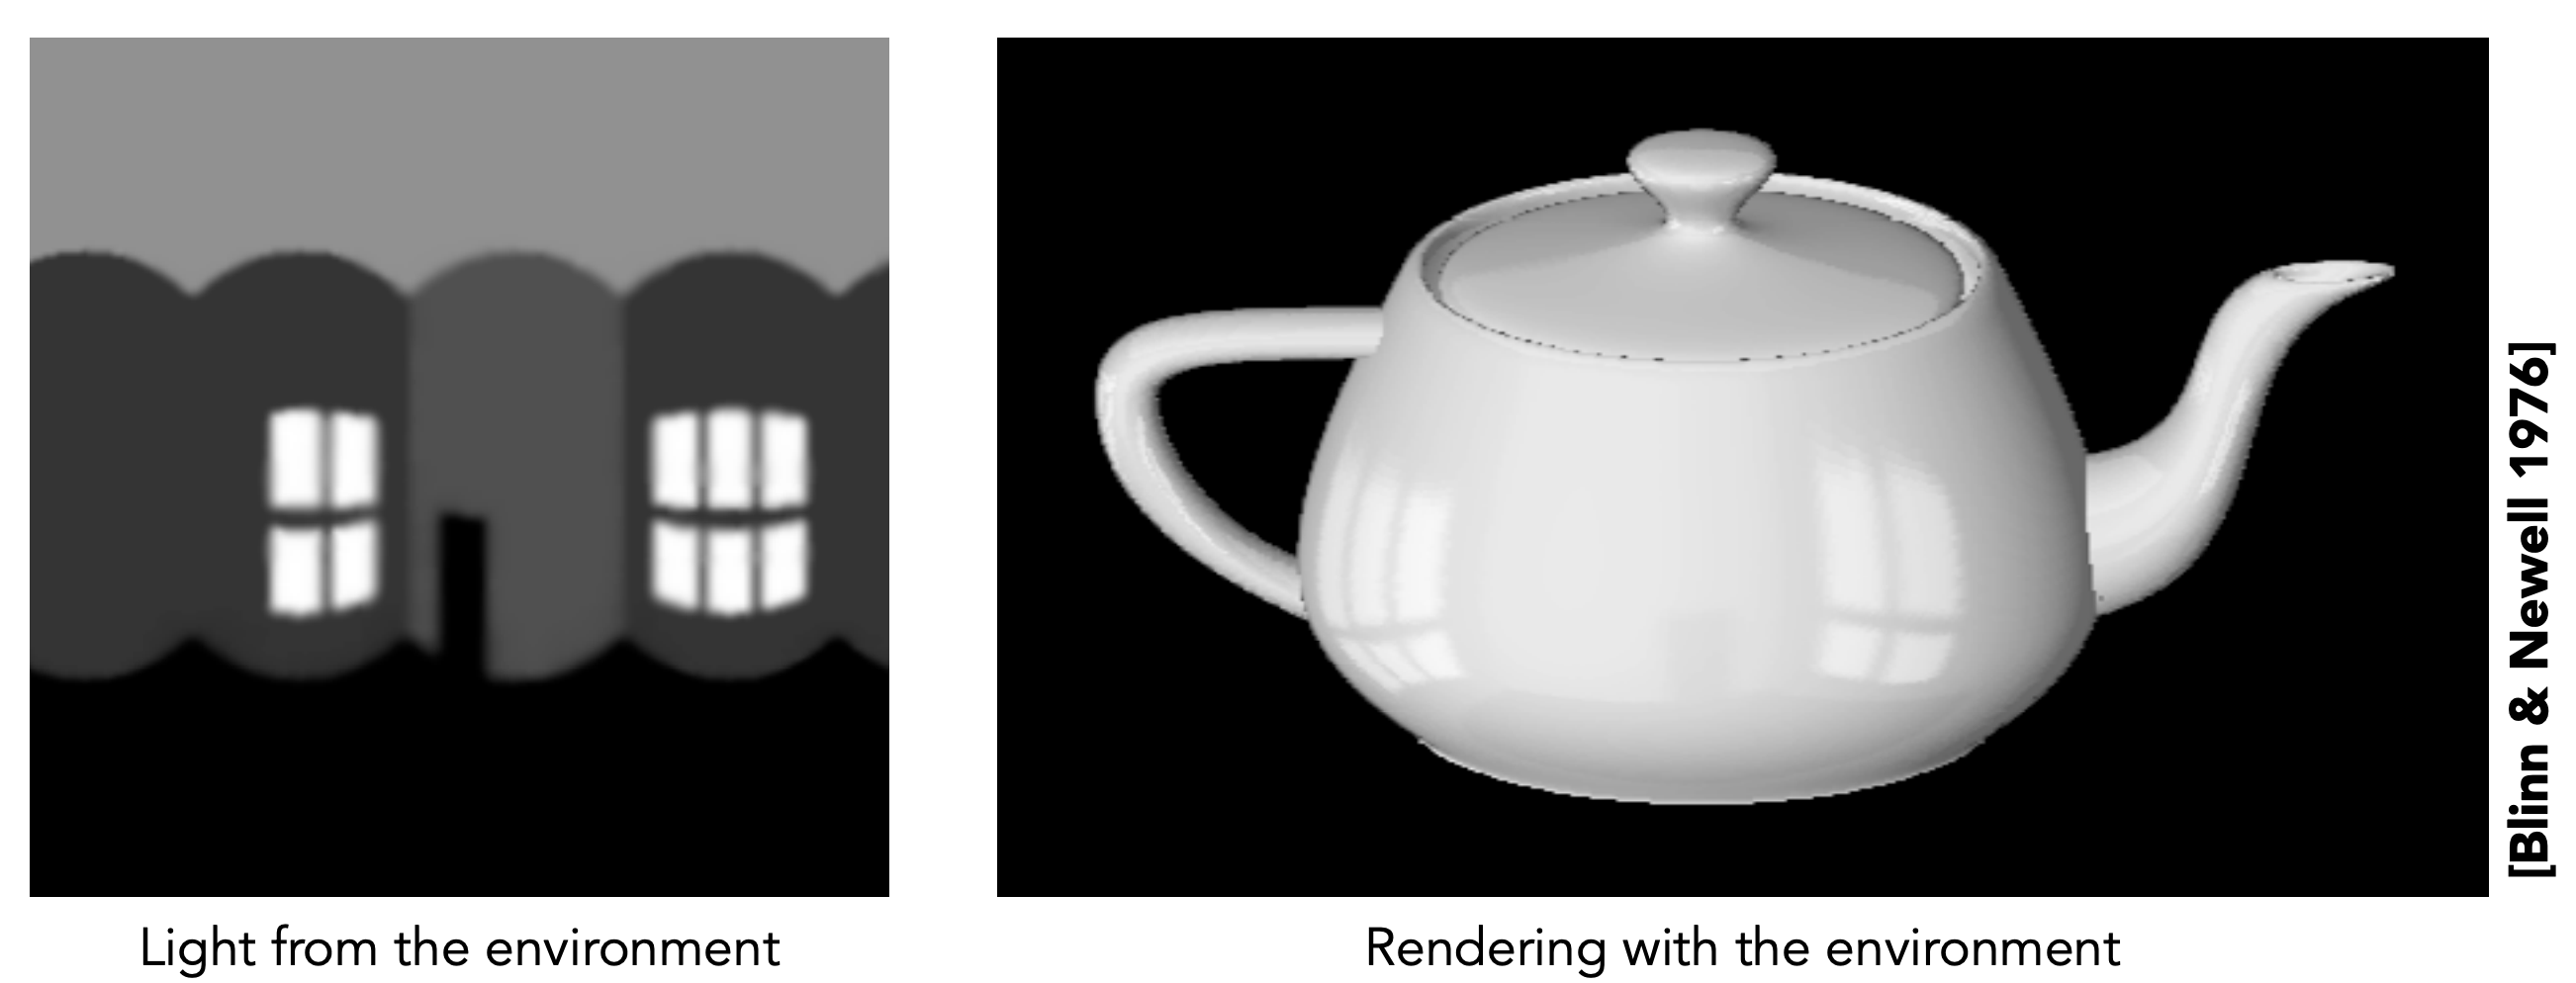
\includegraphics[scale=.2]{huanjingtietu.png}
	\caption{环境贴图示意}
	\label{fig:huanjingtietu}
\end{figure}
\begin{enumerate}
	\item 墨卡托投影法 (Mercator Projection) : 通过将球面映射到一个平面上, 我们可以使用墨卡托投影法. 墨卡托投影法应用于目前地球仪的投影. 它的特点是靠近南北极的地方会发生较大的畸变, 这不是一个均匀地描述. 
	\begin{figure}[H]
		\centering
		\includegraphics[scale=.2]{mokatuo.png}
		\caption{墨卡托投影法}
		\label{fig:mokatuo}
	\end{figure}
	\item 立方体映射 (Cube Map) : 我们为光滑球定义一个包围盒, 将球的平面投影到立方体的六个平面上. 这样做就可以得到6张纹理, 并且畸变比较小. 但是在计算纹素时需要计算球面上的点对应哪一张纹理, 判断点和方向的位置关系. 
	\begin{figure}[H]
	\centering
	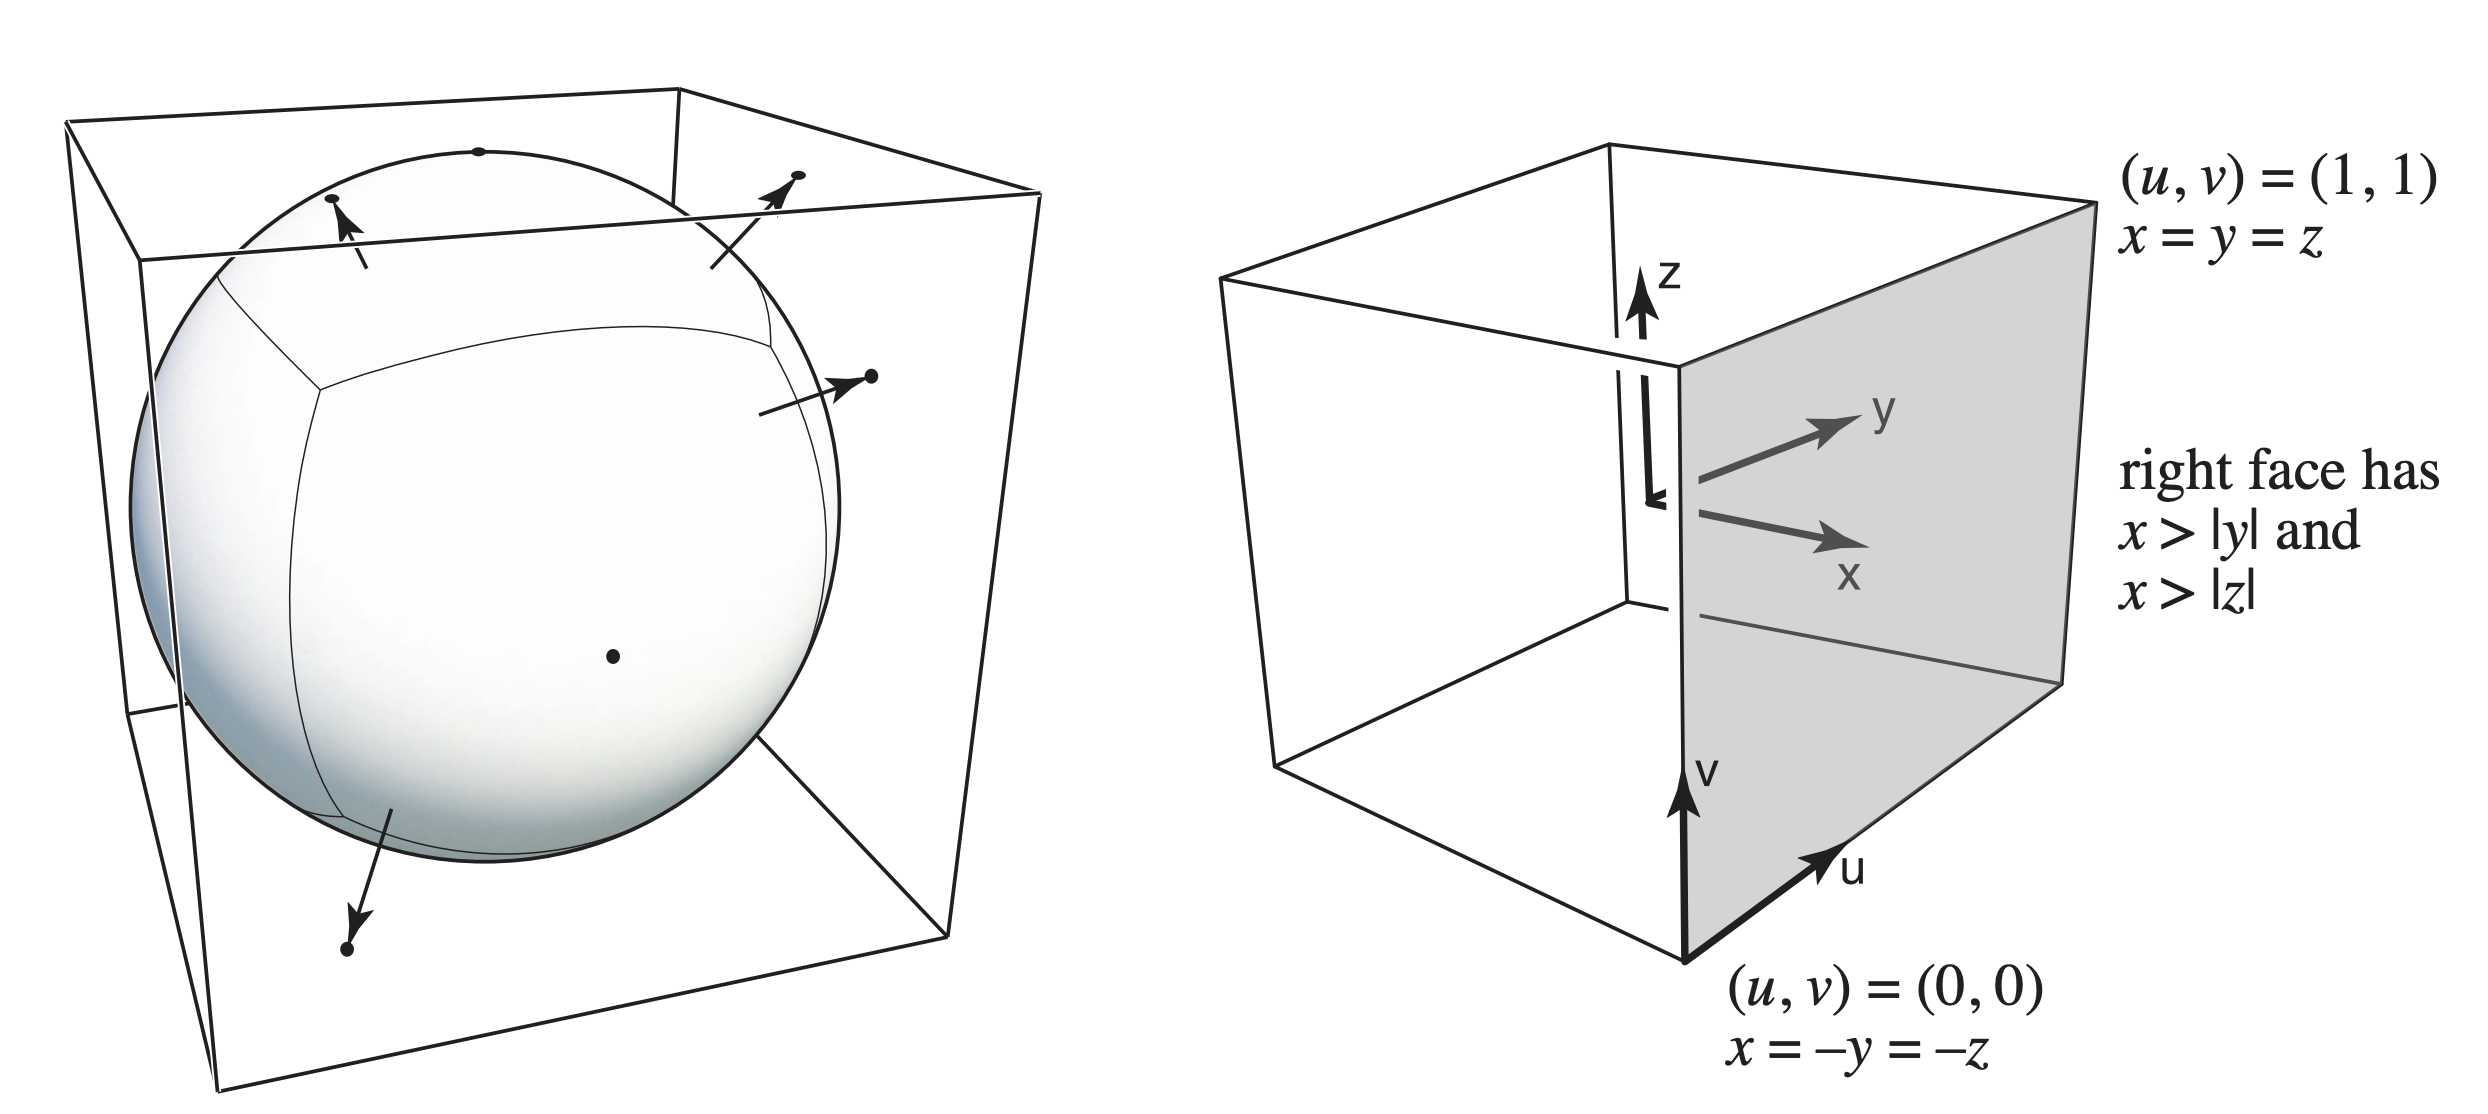
\includegraphics[scale=.15]{cubemap.png}
	\caption{立方体映射}
	\label{fig:cubemap}
	\end{figure}
\end{enumerate}

\subsection{凹凸贴图}
\textbf{凹凸贴图}是指用纹理的方式得到物体表面凹凸不平的感觉, 相比于直接通过做出物体凹凸不平的方式, 这种方法更加的简单. 对于任何一个点, 我们只需要改变这个点的法线方向就可以表达出这个点高度的变化. 因此这个贴图也被称作\textbf{法线贴图 (Bump mapping) }. 纹理上的点定义的是点高度的移动, 通过纹理上信息我们可以求出新的法线方向. 

在二维的情况下, 我们假设原物体是一条直线, 原始法线方向为$(0,1)$. 对于任意一个点$p$, 我们定义$p$点的导数是$dp=c\cdot [h(p+1)-h(p)]$. 常数$c$定义了凹凸贴图对于法线的影响. 那么该点切线的方向是$(1, dp)$. 法线的方向和切线的方向成90度角, 法线的方向向量是$(-dp, 1)$正则化后的结果. 
\begin{figure}[H]
	\centering
	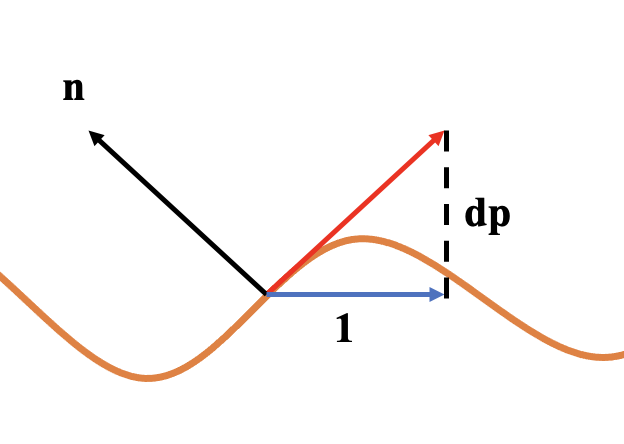
\includegraphics[scale=.5]{aotutietu.png}
	\caption{二维情况下法线贴图中法线的计算}
	\label{fig:aotu}
\end{figure}

推广到三维情况, 对于一个原始法线是$(0,0,1)$的平面, 我们在u方向和v方向上各做一次求导, 结果是$dp/du=c1\cdot [h(u+1)-h(u)],dp/dv=c2\cdot [h(v+1)-h(v)]$. 法线的方向是$(-dp/du,-dp/dv,1)$的正则化结果. 

对于任意方向的原始法线, 我们都可以先按照局部坐标系计算法线后通过变换变换到世界坐标系上. 

除了凹凸贴图之外, 还有另外一种贴图称作\textbf{位移贴图}. 位移贴图会移动所有顶点位置. 因此使用顶点贴图的时候模型三角形分的越细越好. 凹凸贴图并没有实际改变物体的形状, 所以在物体的边上依旧可以看到光滑的曲线. 
\begin{figure}[H]
	\centering
	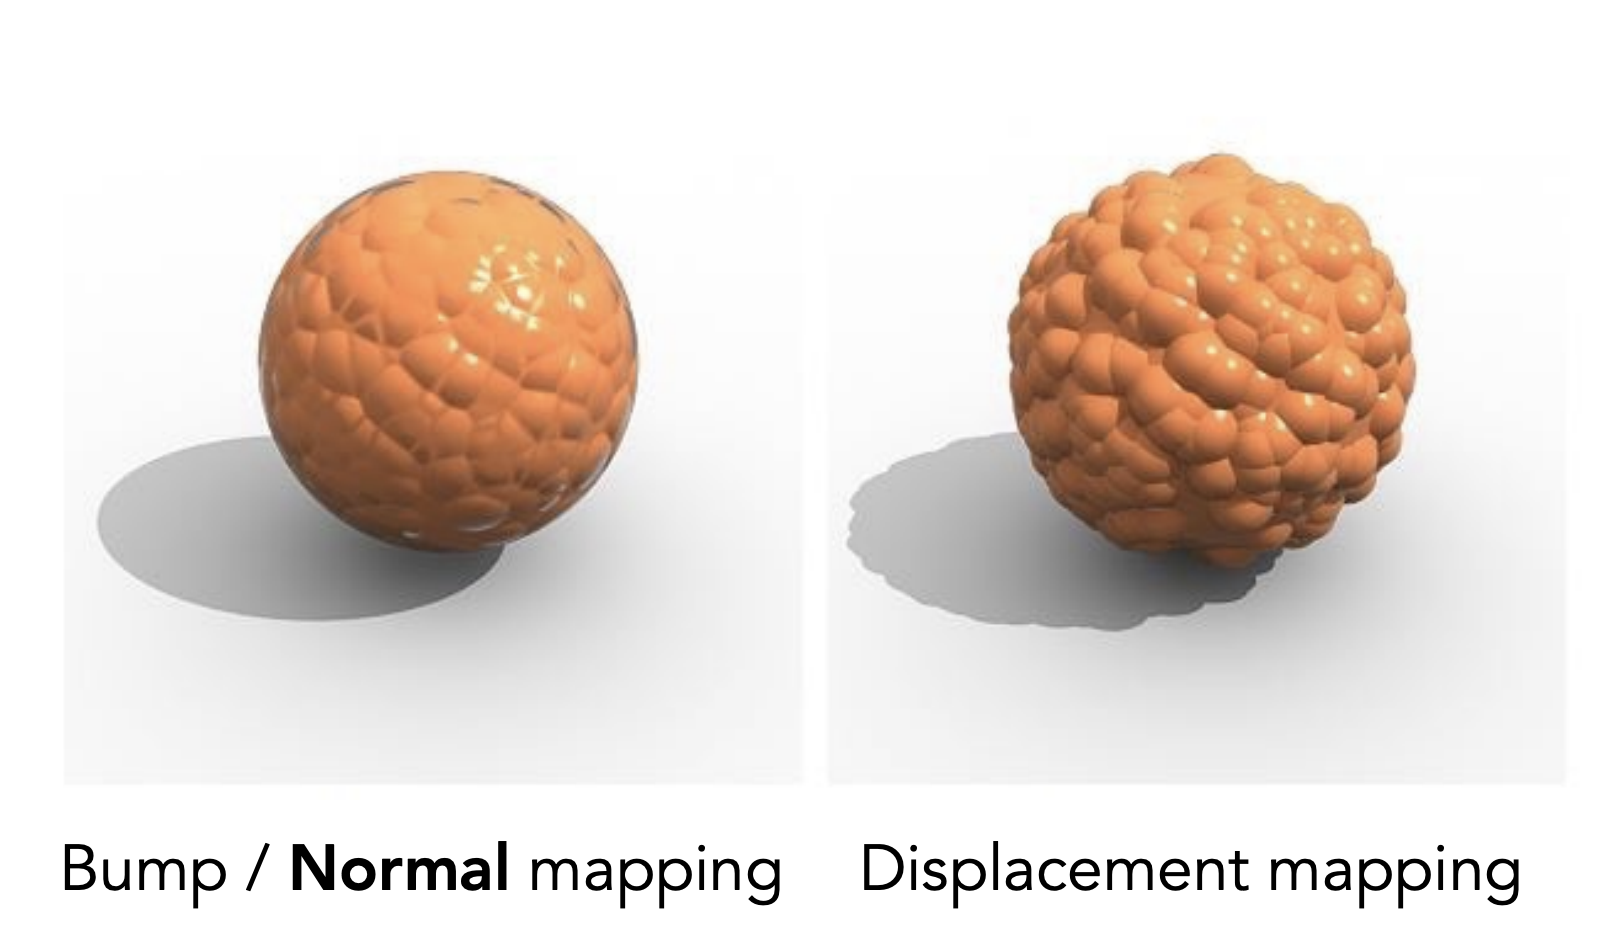
\includegraphics[scale=.3]{weiyitietu.png}
	\caption{凹凸贴图和位移贴图}
	\label{fig:weiyitietu}
\end{figure}

当然, 贴图可以推广到三维空间, 我们可以使用三维贴图. 计算三维空间中任意一个点对应的纹理. 

\section{阴影贴图}
贴图还可以直接加入一些阴影, 直接计算好贴在纹理上, 这样会使得阴影计算变得很快. 纹理可以记录一些已经计算好阴影的信息. 
